\documentclass{article}
\usepackage{graphicx}
\usepackage{subcaption}
\usepackage{amsmath}
\usepackage{pgfplots}
\usepackage[margin=25truemm]{geometry}

\title{CSCI2750 Homework 1}
\author{Wong Cheuk Yin 1155192671}
\date{\today}

\begin{document}
    \maketitle 
    \section{Problem 1}
    \subsection{Part (a)}
    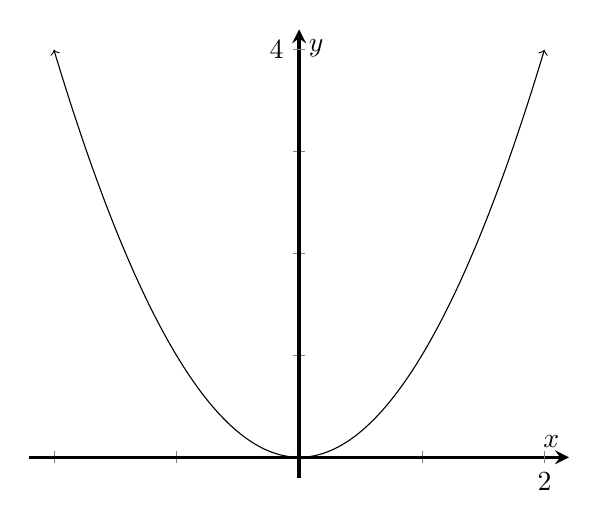
\begin{tikzpicture}
    [baseline=(current bounding box.north)]
    \begin{axis}[
    xmax=0, xmax=20,
    ymin=-6, ymax=6,
    axis lines=middle,
    axis line style={very thick},
    xticklabels={},
    yticklabels={},
    xtick distance=1, ytick distance=1,
    extra x ticks=2, extra y ticks=4,
    xmin=-2.2, xmax=2.2,
    ymin=-0.2, ymax=4.2,
    xlabel=$x$,
    ylabel=$y$]
    \addplot[<->,domain=-2:2,samples=500](x,{x^2});
\end{axis}
\end{tikzpicture}

\end{document}